\documentclass[french]{article}
\usepackage{geometry}
\geometry{a4paper}
\usepackage{graphicx}
\usepackage{amssymb}
\usepackage{amsmath}
\usepackage{amsthm}
\usepackage{empheq}
\usepackage{mdframed}
\usepackage{booktabs}
\usepackage{graphicx}
\usepackage{color}
\usepackage{psfrag}
\usepackage{pgfplots}
\usepackage{bm}
\usepackage[utf8]{inputenc}
\usepackage[T1]{fontenc}
\usepackage{babel}
\usepackage{indentfirst}
\usepackage{float}
\usepackage{enumitem}
\usepackage{subcaption}
\usepackage{hyperref}




\definecolor{ocre}{RGB}{243,102,25}
\definecolor{mygray}{RGB}{243,243,244}

\newcommand\orangebox[1]{\fcolorbox{ocre}{mygray}{\hspace{1em}#1\hspace{1em}}}

\newtheoremstyle{mytheoremstyle}
    {3pt}
    {3pt}
    {\normalfont}
    {0cm}
    {\rmfamily\bfseries}
    {.}
    {1em}
    {{\color{ocre}\thmname{#1}~\thmnumber{#2}}\thmnote{\,--\,#3}}
\newtheoremstyle{myproblemstyle}
    {3pt}
    {3pt}
    {\normalfont}
    {0cm}
    {\rmfamily\bfseries}
    {.}
    {1em}
    {{\color{black}\thmname{#1}~\thmnumber{#2}}\thmnote{\,--\,#3}}
\theoremstyle{mytheoremstyle}
\newmdtheoremenv[
    backgroundcolor=mygray,
    linecolor=ocre,
    leftmargin=0pt,
    innerleftmargin=20pt,
    innerrightmargin=20pt,
]{theorem}{Theorem}[section]
\theoremstyle{mytheoremstyle}
\newmdtheoremenv[
    backgroundcolor=mygray,
    linecolor=ocre,
    leftmargin=0pt,
    innerleftmargin=20pt,
    innerrightmargin=20pt,
]{definition}{Definition}[section]
\theoremstyle{myproblemstyle}
\newmdtheoremenv[
    linecolor=black,
    leftmargin=0pt,
    innerleftmargin=10pt,
    innerrightmargin=10pt,
]{problem}{Problem}[section]

\usepgfplotslibrary{colorbrewer}
\pgfplotsset{width=8cm,compat=1.9}

\title{Approches Deep Learning à la détection d'anomalies dans un système à temps réel}
\author{Mohamed-Amine ROMDHANE, Adam BOND\\Encadré par: Pr. Enrico Formenti}
\date{}


\begin{document}
    \maketitle

    \tableofcontents
    \clearpage
    

    \section{Introduction}
    Dans le cadre d'un besoin d'une startup spécialisée dans des services d'optimisation de consommation d'eau dans le milieu agricole, on veut pouvoir mettre en place un modèle de détection d'anomalies matérielles via des méthodes d'apprentissage automatique et d'intelligence artificielle. Dans cette optique, cette entreprise a installé des senseurs sur des pompes à eaux qui en indiquant la pression à l'intérieur, permettent d'indiquer l'état d'irrigation actuel. L'irrigation est déclenchée automatiquement à l'aide de capteurs d'humidité du sol.     
    \section{Problématique \& Hypothèses}
    Les senseurs de pression d'eau d'une pompe ne sont pas parfaits, et ils peuvent envoyer des valeurs légèrement différentes entre deux lectures à cause du bruit statistique. De plus, certains facteurs comme la chaleur ou l'humidité qui varient naturellement font en sorte que les courbes de ces senseurs ont toujours un bruit de basse amplitude. Il peut aussi arriver qu'une bulle d'air ou un petit objet passe temporairement par la pompe et devienne une "dent" sur le graphe de suivi de pression d'eau, c'est à dire une forte perturbation d'amplitude en un court moment.
    \newline
    \indent Le fonctionnement normal d'une pompe ressemble donc à une période calme perturbée uniquement par un bruit statistique global, puis lorsque le capteur détecte que l'irrigation est nécessaire la courbe grimpe jusqu'à son maximum, et y reste jusqu'à ce que le capteur détecte que la terre est suffisamment irriguée. S'ensuit une chute de la pression puis un retour au calme jusqu'au prochain cycle.
    \newline
    \indent Dans le cadre de cette étude, deux problèmes se sont posés à nous. Le premier est celui de la disponibilité des données, le contact limité avec l'entreprise nous ayant simplement permis d'obtenir des aperçus et non un jeu de données complet. L'autre facteur est la complexité de la modélisation, étant donné qu'en réalité les senseurs dépendent d'un grand nombre de variables, les senseurs dépendant les uns des autres et les bruits ainsi que les anomalies ayant plusieurs sources et facteurs. 
    \newline
    \indent Le but de ce projet est donc de développer des approches d'apprentissage profond permettant de détecter automatiquement des malfonctions dans les données de pression des senseurs.
    \section{Les données}
    Afin d'obtenir un jeu de données sur lequel entraîner nos modèles, nous avons choisi d'écrire un simulateur se basant sur les données que l'entreprise nous a communiqué. Cet outil se doit d'être modulaire pour nous permettre de générer des données correspondant à la bonne marche d'un senseur ou à une malfonction en prenant en compte autant de facteurs auxquelles l'entreprise est confrontée que possible; par exemple l'amplitude moyenne ou le type de bruit, l'amplitude maximum en fonction des senseurs, la durée de chaque état, ou encore la nature des transitions entre chaque état.
        \subsection{Simulation des données}
        Le simulateur \textit{simulator.py} simule un système à temps réel, c'est à dire un système qui contrôle un objet (ici les pompes à eau) en modifiant son comportement en temps réel en fonction de nouvelles données. Ainsi la pompe doit commencer à irriguer si elle détecte par exemple que la terre n 'est pas assez humide. En fonction des décisions prises par ce système à temps réel, les résultats enregistrés par le senseur de pression de l'eau vont être modifiés. Afin de modéliser ce système, nous avons utilisés plusieurs variables:
        \begin{itemize}[label={•}]
            \item \textbf{realtime\_tick} représente l'écoulement temporel en millisecondes avant l'enregistrement d'un échantillon. Cette variable s'incrémente par \textit{dt\_per\_sample} après chaque échantillon.
            \item \textbf{dt\_per\_sample} est le temps en secondes entre chaque étape de simulation (temps entre deux échantillons).
            \item \textbf{transition\_type} est le type de transition appliqué entre deux états (exemple: East-In-Out Quad, Ease-In-Out Sine, Linear...). Pour conserver le nombres d'échantillons qu'on a, pour un état $A$ et $B$ où la différence d'amplitude est importante, on prend par exemple, les $n$ derniers échantillons de $A$ et et les $n$ premiers échantillons de $B$ et on applique la fonction de transition les $2n$ échantillons.
            \item \textbf{noise} est la fonction de bruit global présent dans le système (exemple: "gaussian" pour un bruit gaussien). Le bruit a sa propre amplitude. 
            \item \textbf{states} est la liste d'états. Chaque état a une durée, une amplitude, et une liste (vide ou non) d'anomalies (appelées impulsions dans le contexte de simulation). Une \textit{anomalie} a sa propre durée, le temps de son début ainsi que son amplitude.
        \end{itemize}
        \subsection{Génération des données}
    \section{Deep Learning avec TensorFlow}
        \subsection{Approche naïve avec CNN}
       En premier lieu nous avons essayé d'utiliser le réseau neuronal convolutif de TensorFlow (convolutional neural networks, abbrv: cnn) pour l'entraîner à reconnaître les images provenant d'un système stable ainsi qu'un système à forte perturbations admettant plusieurs anomalies. Nous avons essayé de l'entraîner sur des images car c'est comme que cela que ça fonctionne actuellement dans l'entreprise; un employé regarde défiler les courbes à la recherche de malfonctions. Nous avons précédemment généré 1000 images pour chacune de nos classes \textbf{stable} et \textbf{malfunction}, nous les avons alors importées pour être pré-traitées avant de les brancher au réseau.
       
       Parmi les étapes du pré-traitement, nous avons redimensionne la taille de l'image (originalement 640x480) à 250x250. Étant donné que la couleur de l'image n'a pas d'importance, nous avons restreint les couleurs à du noir et blanc. Cette manipulation a le bénéfice d'avoir un \emph{tensor} de dimension (250x250x1) au lieu de (250x250x3). Nous avons défini le nombre d'\emph{epochs} comme étant égal à 10 et le nombre de \emph{batchs} de données à être traités simultanément dans le réseau de neurones à 10 également. Notre modèle TensorFlow a le \emph{pipeline} décrit ci-dessous:
        \begin{center}
            Une \textbf{couche de convolution} à 2 dimensions avec \textbf{16} filtres, un noyau de taille \textbf{3x3} et la fonction de correction \textbf{RELu}. \\
            $
            \downarrow
            $\\
            Une \textbf{couche de pooling} où on prend que le \textbf{maximum} à l'issue des résultats précédents. \\
            $
            \downarrow
            $\\
            Une \textbf{couche de convolution} à 2 dimensions avec \textbf{32} filtres, un noyau de taille \textbf{3x3} et la fonction de correction \textbf{RELu}. \\
            $
            \downarrow
            $\\
            Une \textbf{couche de pooling} où on prend que le \textbf{maximum} à l'issue des résultats précédents. \\
            $
            \downarrow
            $\\
            Une \textbf{couche de convolution} à 2 dimensions avec \textbf{64} filtres, un noyau de taille \textbf{3x3} et la fonction de correction \textbf{RELu}.\\
            $
            \downarrow
            $\\
            Une \textbf{couche entièrement connectée} avec \textbf{512} neurones et une fonction d'activation \textbf{RELu}.\\
            $
            \downarrow
            $\\
            Une seul neurone avec la fonction d'activation \textbf{Sigmoïd}.
        \end{center}
        Avec 
        \[
        RELu(x) = \begin{cases}
            x,& \text{si } x \ge 0\\
            0,& \text{sinon}
        \end{cases}
        \]
        et
        \[
        Sigmoid(x) = \dfrac{1}{1+e^{-x}}
        \]
        \begin{figure}[H]
            \centering
            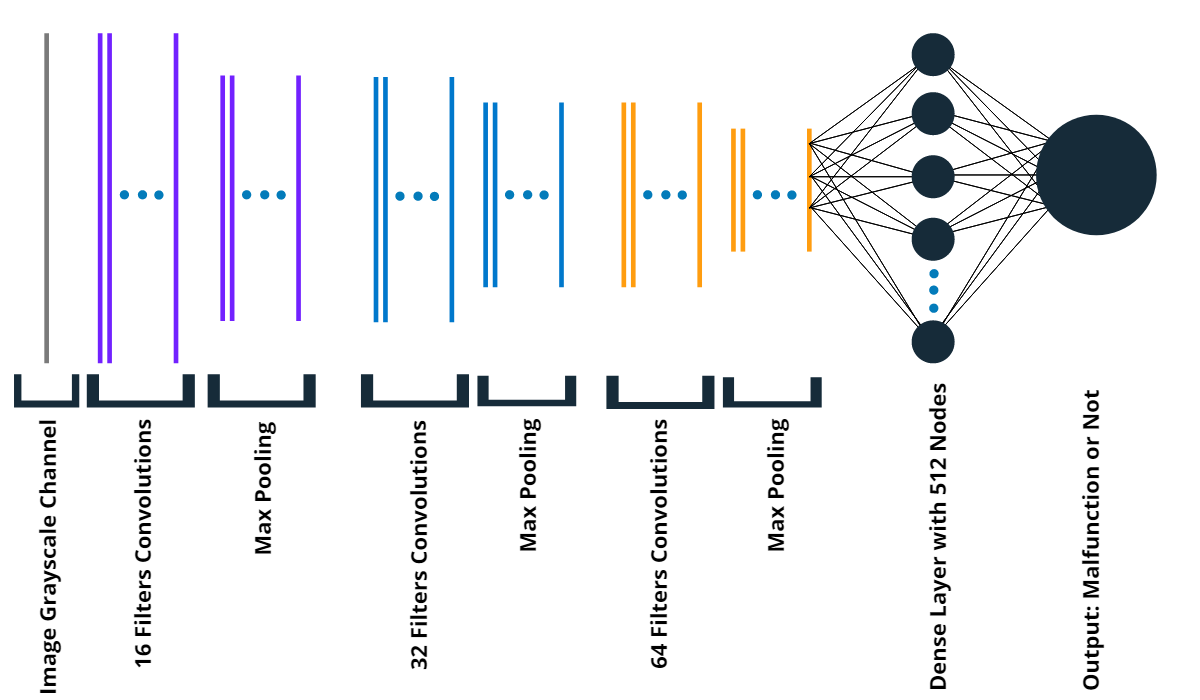
\includegraphics[width=\textwidth]{images/cnn.png}
            \caption{Le modèle CNN de classification d'anomalies}
            \label{}
        \end{figure}
        Notre modèle est compilé avec 2 ensembles d'images distincts. Un ensemble d'images d'entraînement et un ensemble de validation. Au total, nous avons généré 2200 images pour l'entraînement et 2200 images pour la validation.
        \newline
        \begin{itemize}
            \item L'ensemble d'entraînement comporte 1100 images étiquetées \textbf{stable} ainsi que 1100 images étiquetées \textbf{malfunction}.
            \item L'ensemble de validation comporte le même nombre d'images pour chacune des deux classes mais des instances différentes de ceux dans l'ensemble l'entraînement.
        \end{itemize}
        Dans la section 5, nous expliquerons les résultats obtenus par cette approche et pourquoi nous l'avons qualifiés de naïve.
        \subsection{Extraction des features avec TSFresh}
        Afin d'accompagner nos méthodes de détection d'anomalies, nous avons cherché à trouver des \emph{features} permettant de détecter avec succès des anomalies dans le but d'avoir un modèle plus compact. Cela nous permettrait d'avoir un modèle qui ne prend non pas chaque pixel individuel de l'image (250*250) mais un nombre limité qui serait plus rapide a traiter. 
        
        Nous avons pour cela utilisé une libraire Python appelée TSFresh. TSFresh est un outil spécialement conçu pour analyser des séries temporelles en calculant un grand nombre de caractéristiques communes aux séries temporelles\cite{tsfreshfeatures}. La librairie cherche par exemple les coefficients de la série de fourier representée par le signal (fft\_coefficient), où bien le pourcentage de valeurs qui sont présente plus d'une fois, etc. Une fois ces features calculées, TSFresh utilise chacune des features individuellement en essayant de déterminer son efficacité pour prédire correctement la classification d'une série, et lui assigne une p-value en conséquence. La p-value représente la probabilité qu'en supposant l'hypothèse nulle (c'est à dire en supposant que rien n'a changé entre les deux échantillons), on obtienne une valeur égale ou plus grande à cell observée. En pratique, plus la p-value est basse, plus il y a de chances pour qu'une feature soit significative dans la prédiction de malfonctions. En fonction de cette p-value, un algorithme statistique décide de qualifier cette feature comme pertinente ou non.
        
        \begin{figure}[H]
            \centering
            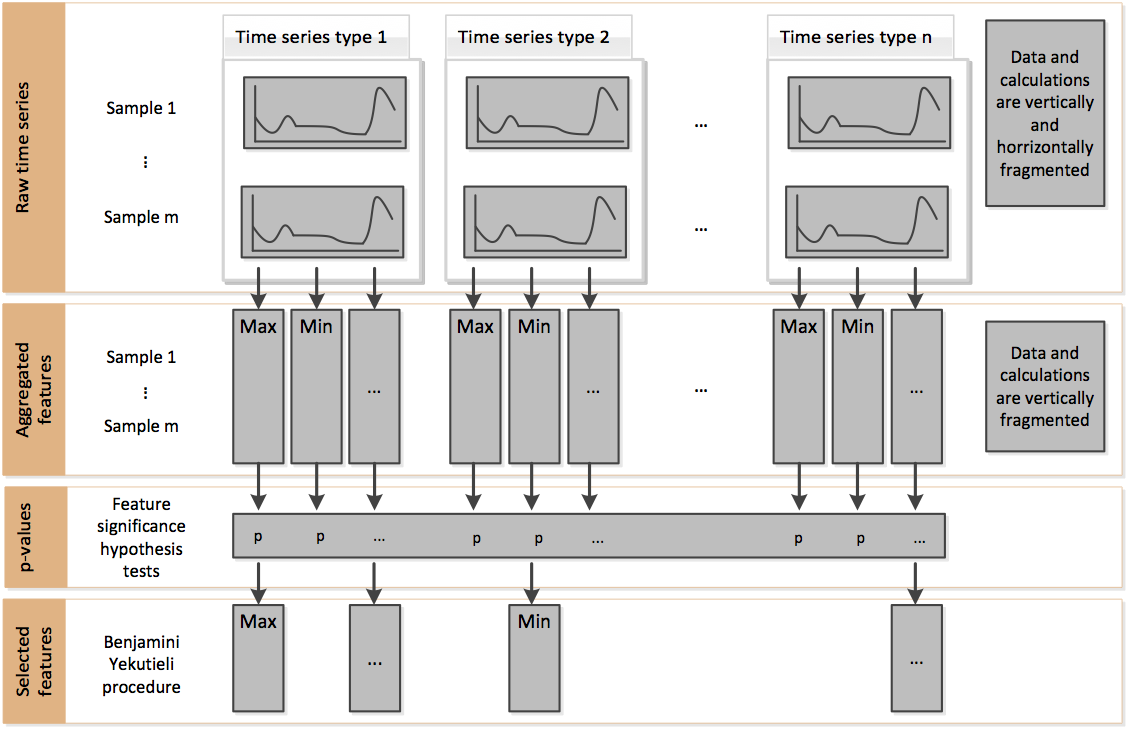
\includegraphics[width=.8\textwidth]{images/features_extraction.png}
            \caption{Image de la documentation TSFresh permettant de visualiser la sélection de features à partir des séries temporelles en entrée.}
            \label{}
        \end{figure}
        
        
        Nous avons d'abord tenté de réaliser cette analyse sur une matrice de pixels représentant l'image. Ainsi à chaque moment T équivaut une colonne de pixels blancs ou rouge, tous les pixels inférieurs à la valeur de l'amplitude étant coloriés en rouge et les autres laissés blancs. Nous avons rapidement abandonné cette idée puisqu'en plus de ne pas apporter plus d'informations par rapport à une simple série où équivaut à chaque moment T une valeur d'amplitude, elle apporte énormément d'informations superflues que TSFresh doit trier, et qui ralentissent le processus et rendent les résultats moins efficaces. Nous avons donc implémenté dans le simulateur un moyen d'exporter dans un fichier texte de nombreuses séries générées aléatoirement et identifiées selon si elles présentent des anomalies ou non.
        
        Une fois cela réalisé, nous avons donné les 1024 séries résultantes au logiciel pour calculer les coefficients. TSFresh a calculé plus de 800 features, dont il a considéré 305 commes pertinentes.
        
\begin{figure}[H]
            \centering
            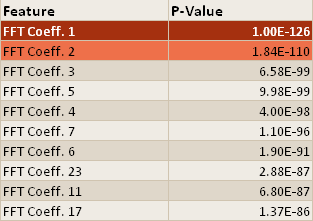
\includegraphics[width=0.35\textwidth]{images/features_pvalue.png}
            \caption{Table des p-value des 10 features les plus significatives.}
            \label{}
        \end{figure}

        Parmi les 305 features, plus de la moitié étaient des coefficients d'une transformée de Fourier, et 48 parmi les 50 premières. Comme on peut le voir sur la table, les premières features et particulièrement la toute première, ont des p-value extrêmement basses, un ordre de grandeur plus petites que les suivantes.
        
        Nous avons vérifié la pertinence de ces features en entraînant deux arbres de décision pour classer les séries temporelles en entrée dans deux classes : stable et malfonction.
        
        Nous avons donné au premier arbre de décision les données brutes, et il a obtenu une précision de 85\% sur les données de test. Nous avons donné aux second arbre uniquement les features extraites par TSFresh et la précision est montée à 90\%.
        
        Nous avons alors décidé de tester ces résultats en comparant la précision d'arbres de décisions qui prendraient uniquement en compte les N premières features afin d'essayer d'obtenir un ensemble de features aussi restreint que possible pouvant rendre la prédiction rapide. 
        
        Les résultats obtenus ont été que bien qu'une tendance se dégage à une plus grande précision plus on prend de features, la différence n'est pas énorme. On obtient 90\% de précision avec les 100 premières features (soit autant qu'avec les 305 features pertinentes), mais la précision est déja de 85\% avec uniquement la première feature, et de  89\% avec les cinq premières.
        
        Afin de limiter l'overfit nous avons aussi vérifié et limité la profondeur maximum des arbres de décisions, mais nous nous sommes rendu compte qu'en réalité même avec toutes les features pertinentes, la profondeur de l'arbre ne dépassait jamais 18. C'est à dire que dans tous les cas, l'arbre de décision choisit d'utiliser un nombre restreint de features.
        
        Ces résultats confirment l'impact énorme des premiers features sélectionnés qui ont des p-values étant plus petites d'un ordre de grandeur.
    
        \subsection{Détection d'anomalies en tant qu'objets}
        Afin de couvrir un large éventail d'approches pour détecter des anomalies, nous avons cherché des techniques plus récentes pour traiter les deux thèmes de ce travail de recherche: \emph{détection d'anomalies} et \emph{temps réel}. Parmi les méthodes pertinents à notre projet, nous avons choisi d'implémenter la détection d'objets. La détection d'objets consiste à identifier une classe d'objets (cercles, visages, signalisation, et dans notre cas des malfonctions) dans une image\cite{odwikipedia}. On peut voir dans la figure ci-dessous un exemple d'une telle détection d'objets réels.
        \begin{figure}[H]
            \centering
            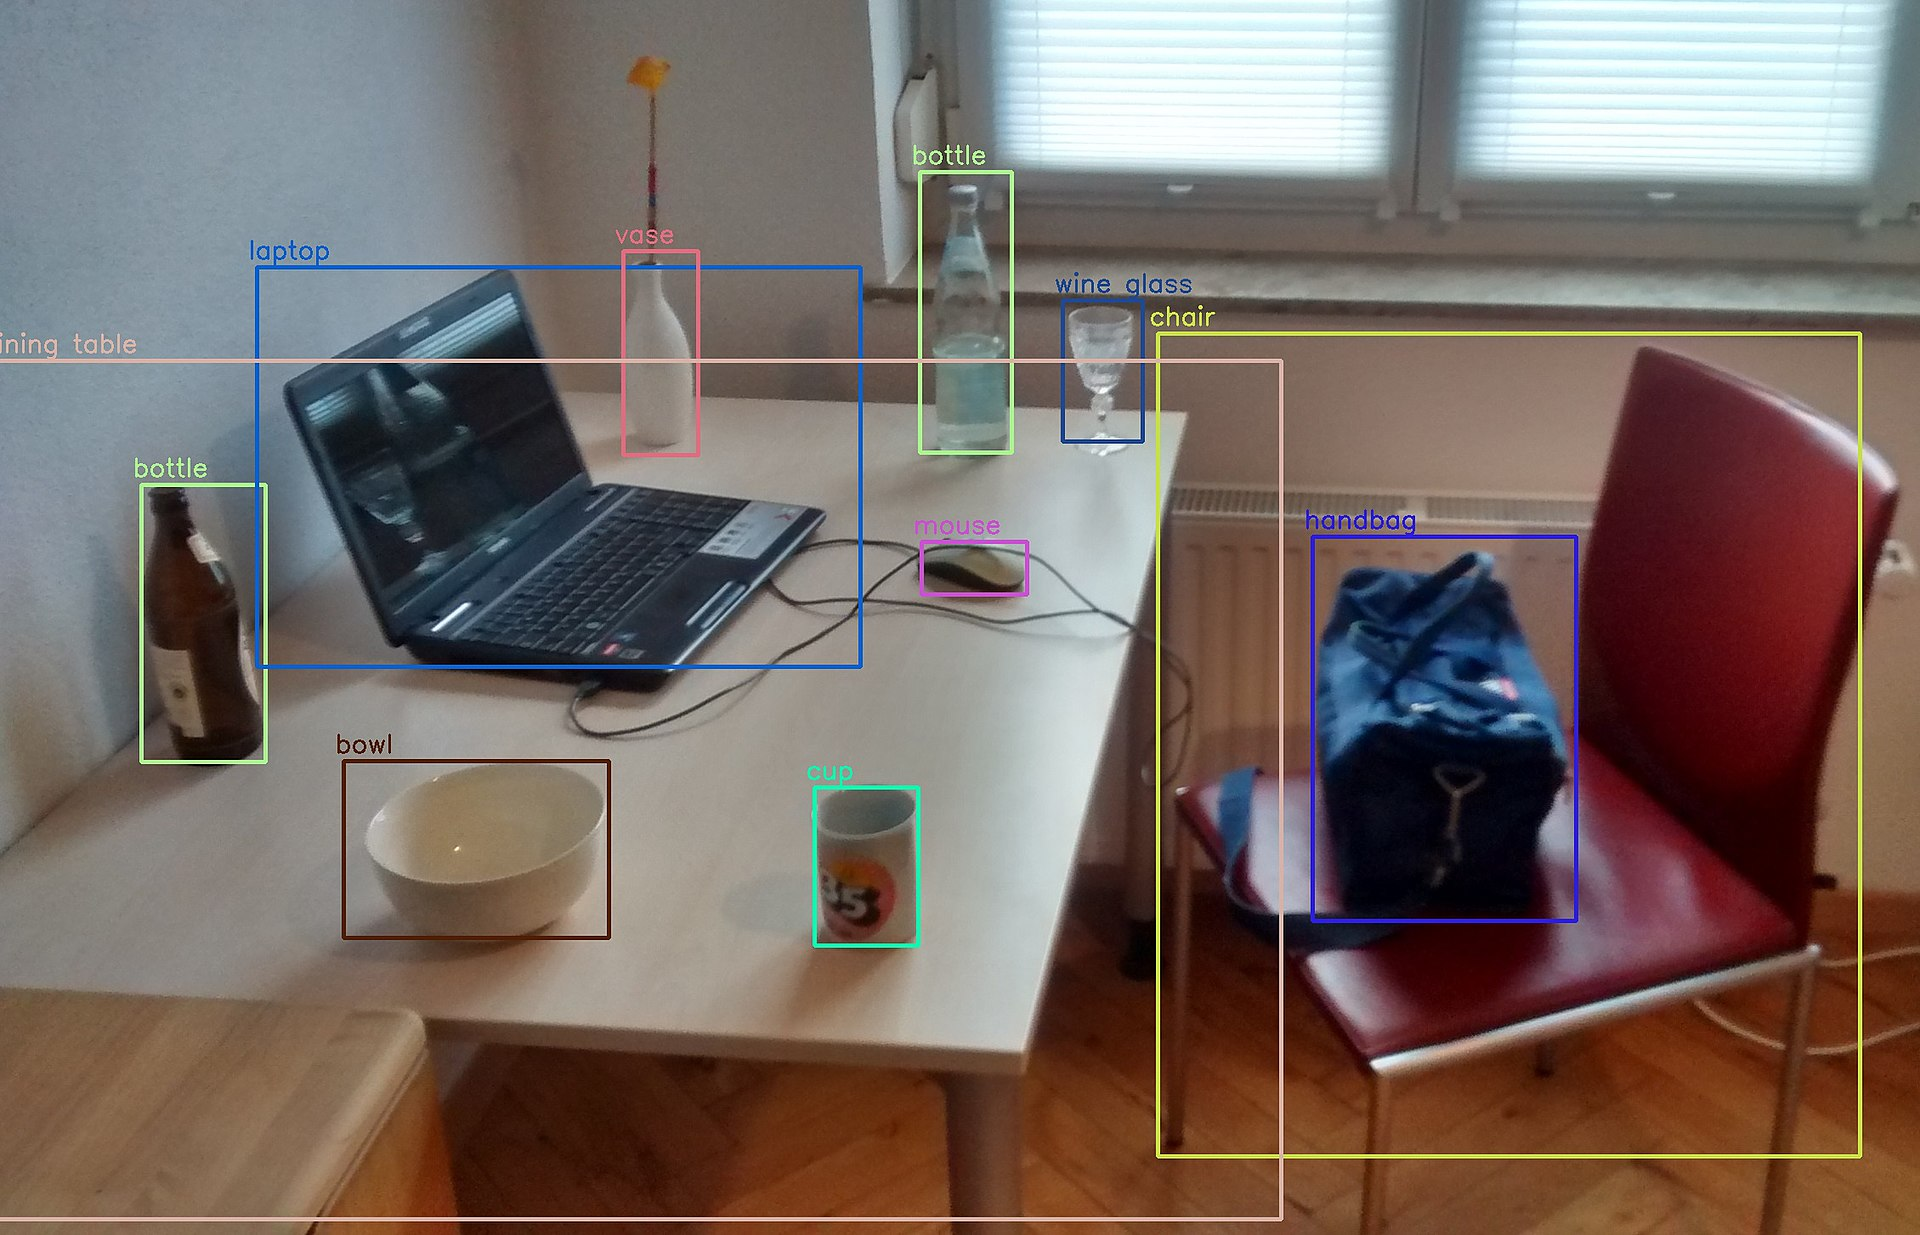
\includegraphics[width=1\textwidth]{images/real_objects.jpg}
            \caption{Image wikipédia qui montre les résultats obtenus d'une détection d'objets à l'aide de l'algorithme YOLOv3 (You Only Look Once) ainsi que le module DNN d'OpenCV. Ce modèle peut détecter jusqu'à 80 objets.}
            \label{}
        \end{figure}
        L'avantage que présente cette méthode est de permettre de reconnaître des objets en temps réel dans, par exemple, une vidéo, ce qui correspond à la méthode employée actuellement par l'entreprise. Dans cette partie, nous allons expliquer la manière dont on génère les données qui servent comme entrée pour un modèle pré-entraîné fourni par l'\emph{API} de détection d'objets de TensorFlow.
        \subsubsection{Une anomalie est un objet}
        Après avoir consultés la documentation de l'\emph{API} de détection d'objets, nous avons constaté que celle-ci demande un format très particulier (un fichier binaire TFRecord) ainsi qu'une configuration complexe (un fichier .config avec les configurations possibles du modèle). Les anomalies présentes dans une image doivent être identifiées et isolées chacune dans sa propre \emph{bounding box}, c'est à dire le rectangle le plus petit à l'intérieur duquel tous les points de l'anomalie sont présents. L'outil qui permet de faire cette manipulation s'appelle \emph{LabelImg}. Cet outil permet de générer un fichier \emph{csv} comportant les colonnes suivantes: \textbf{filename} (le nom de fichier d'image où l'anomalie se trouve), \textbf{width} (la largeur de l'image), \textbf{height} (la hauteur de l'image), \textbf{class} (la classe/libellé/étiquette de l'image, \emph{malfunction} dans notre cas), et les coordonnées des quatre points définissant les coordonnées de la \emph{bounding box} : \textbf{xmin, ymin, xmax, ymax}. Le problème s'est cependant posé de la génération d'une  base de données conséquente d'anomalies isolées. L'automatisation de ce processus étant complexe et sa génération manuelle coûteuse en temps, nous avons décidé de chercher méthode pour résoudre ce problème.
        \begin{figure}[H]
            \centering
            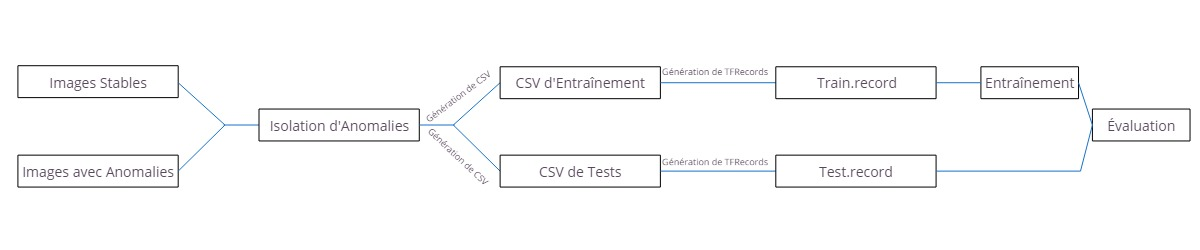
\includegraphics[width=\textwidth]{images/od_datagen.jpg}
            \caption{Pipeline de génération de données pour l'entraînement du modèle de TensorFlow Object Detection API}
            \label{}
        \end{figure}
        \indent Étant donné que nous avons une version stable d'un système à temps réel ainsi qu'une version avec des anomalies, à l'aide de la librairie de traitement d'images OpenCV nous procédons aux traitements suivants:
        \newline
        Soit une simulation $S$ d'un système à temps réel commençant à un temps $t$, ayant une durée $d$. On capture la courbe d'état des deux version (stable et avec anomalies) de $t$ à $t+d$ en tant qu'image (Figure 6.a et 6.b respectivement).
        \newline
        Soit $M_{stable}$ la matrice de pixel de l'image du système stable capturée, et soit $M_{malfunction}$ la matrice de ce même système mais avec une forte présence d'anomalies.
        L'algorithme est le suivant:
        \begin{enumerate}
            \item $M_{diff} = M_{stable} - M_{malfunction}$
            \item On applique 2 fois le filtre \textbf{erode} d'OpenCV (érosion) sur $M_{diff}$ pour se débarrasser des petits clusters de pixels. On a une petite perte d'information sur cette étape qui se compense sur le fait de négliger les anomalies de taille moins importante dû à une erreur de lecture peu fréquente, par exemple.
            \item On applique la fonction \textbf{inRange} d'OpenCV pour obtenir le masque d'image $Mask$ qui extrait les pixels ayant une valeur entre deux gammes de couleurs. Pour notre cas, vu que nos images sont presque similaires, la matrice de pixels $M_{diff}$ admet des couleurs entre le noir et le blanc, le noir étant la couleur de fond et le blanc est le résidu issue de la soustraction. Le masque capture ce résidu.
            \item On applique la fonction \textbf{findContours} d'OpenCV, qui renvoie la liste des contours (bounding box) de chaque cluster de résidu dans $Mask$.
            \item Pour chaque contour trouvé, on extrait le rectangle minimal qui enveloppe ce contour avec la fonction \textbf{boundingRect} d'OpenCV.
            \item Pour chaque \textbf{bounding box}, on écrit la ligne correspondante dans un fichier \textbf{csv} avec les données mentionnées précédemment.
        \end{enumerate}


\begin{figure}[H]
    \centering
    \begin{subfigure}[t]{0.3\textwidth}
            \centering
            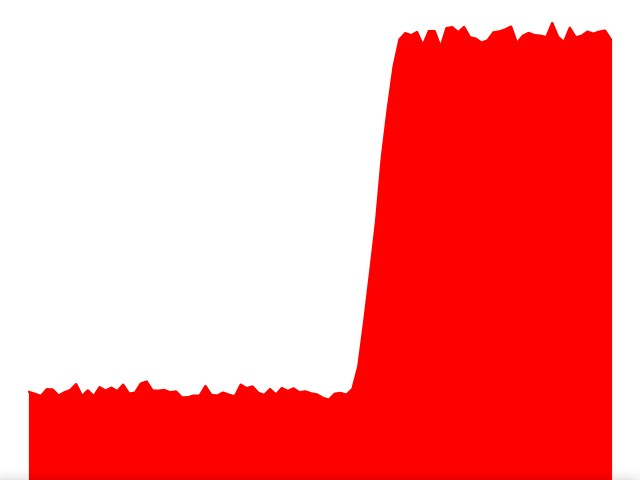
\includegraphics[width=1\linewidth]{images/od_stable.jpg}
            \caption{Figure A}
    \end{subfigure}%
    \begin{subfigure}[t]{0.3\textwidth}
            \centering
            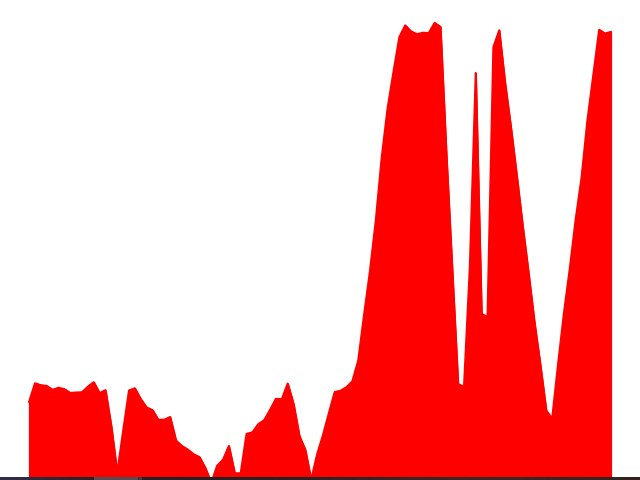
\includegraphics[width=1\linewidth]{images/od_malfunction.jpg}
            \caption{Figure B}
    \end{subfigure}
    \begin{subfigure}[t]{0.3\textwidth}
            \centering
            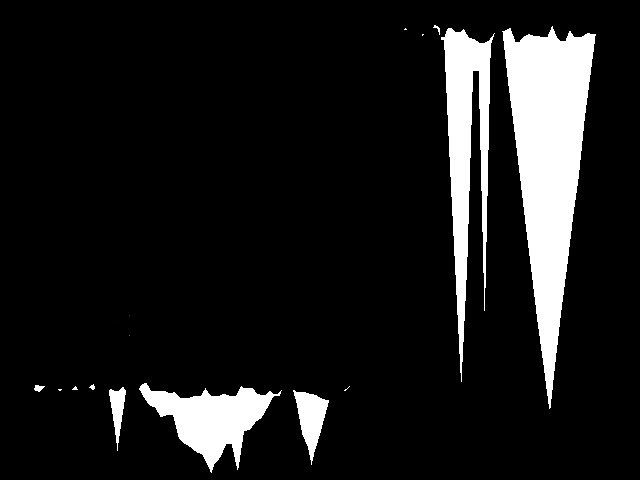
\includegraphics[width=1\linewidth]{images/od_isolated.jpg}
            \caption{Figure C}
    \end{subfigure}
    \caption{La figure A représente l'image du système $stable$, la figure B le système $malfunction$ avec des fortes perturbations, et la figure C l'image résultante de l'opération de soustraction des matrices de pixels des deux: $M_{diff}$ (1. de l'algorithme ci-dessus)}
\end{figure}

\begin{figure}[H]
    \centering
    \begin{subfigure}[t]{0.3\textwidth}
            \centering
            
\includegraphics[width=1\linewidth]{images/od_erosion.jpg}
            \caption{Figure A}
    \end{subfigure}%
    \begin{subfigure}[t]{0.5\textwidth}
            \centering
            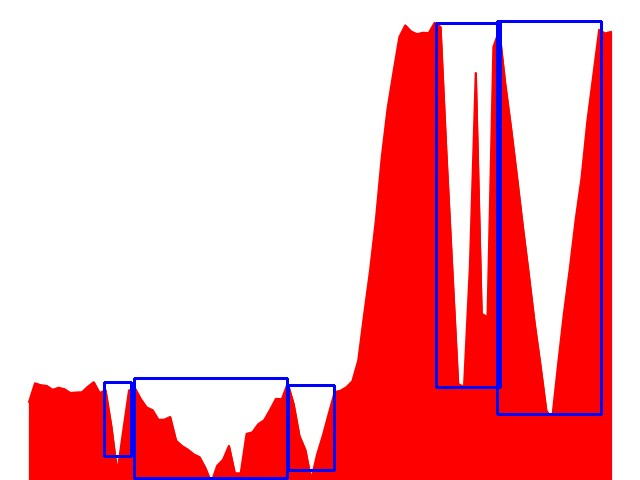
\includegraphics[width=1\linewidth]{images/od_identified.jpg}
            \caption{Figure B}
    \end{subfigure}
    \caption{La figure A représente l'image issue de la matrice de pixel $M_{diff}$ après l'application du filtre d'érosion, et la figure B le résultat des opérations 3, 4 et 5 de l'algorithme ci-dessus.}
\end{figure}

        \subsubsection{Entraînement du modèle}
        L'\emph{API} de détection d'objets de offre plusieurs modèles pré-entraînés. Pour notre entraînement, nous avons opté pour le modèle \textbf{ssd\_mobilenet\_v1\_coco}\cite{pretrainedmodel} qui utilise MobileNet développé par Google. Ce dernier offre une latence de détection de 30ms et un score \textbf{mAP} (mean Average Precision) de 21. Pour la détection d'objets en général, un compromis entre précision et vitesse est à envisager. Après avoir modifié la configuration de ce modèle pour la prise en compte de nos données (les deux fichiers d'entraînement et de test en format TFRecord), nous le lançons avec un nombre de batch de $12$ et un nombre maximal d'itérations de $15 000$ pour ne pas avoir à entraîner le modèle indéfiniment. L'éxecution a été faite avec une machine possédant un processeur Intel i5 avec une fréquance de $2.3GHz$ et une carte graphique NVIDIA GTX960M doté de la technologie CUDA et 8Go de RAM. Sous limite de mémoire, nous avons réussi à n'avoir que 320 \emph{bounding boxes} pour l'exécution du modèle, dont 60 sont des données de test/validation et 260 sont utilisés par le modèle pour du \emph{fine-tuning} d'entraînement. En premier lieu, nous avons essayé de lancer l'entraînement directement sur le processeur. Nous avons alors constaté un écoulement de $12$ secondes entre chaque itération du modèle. Si nous le laissions tourner jusqu'à la fin, cela prendrait à peu près $67$ heures. Nous avons donc finalement opté pour un entraînement sur la carte graphique qui, pour chaque itération, prend $0.5$ secondes soit $3$ heures en total. L'\emph{API} récolte aussi des statistiques concernant le modèle après chaque centaine d'itérations, ce qui allonge à son tour considérablement le temps d'éxecution.
        \newline
        \indent L'entraînement a duré à peu près $11$ heures. Dans la section 5, nous analysons les résultats obtenus par cette méthode et du potentiel de l'utilisation d'une telle technique pour résoudre le problème de l'entreprise.

    \section{Analyses et Interprétations}
    \subsection{Approche naïve avec CNN}
    Le choix des hyperparamètres du modèle était directement influencé par la limite de ce que nos machines personnelles peuvent gérer. Le modèle que nous avons choisi produit 33 millions de paramètres (poids du réseau de neurones + bias). Rajouter une couche de plus avec par exemple 128 filtres est impossible en raison d'un manque de mémoire et produit l'exception \textit{ResourceExhausted}.
    \newline
    \indent Les résultats que nous avons obtenu par cette approche se sont avérés décevants. Le modèle conçu souffrant d'\emph{overfit}. En considérant uniquement les mesures de précision (\emph{accuracy} et \emph{loss}), il peut sembler que le modèle est relativement efficace pour reconnaître les images avec anomalies de celles sans anomalies. En revanche, les résultats sont moins positifs lorsqu'on se conentre sur l'erreur. Ci-dessous les courbes associées à chaque mesure ainsi que leurs corrélations. La fonction de \emph{loss} utilisée est \textit{Binary Cross Entropy} : $BCE(y, \hat{y}) = -\dfrac{1}{N} \sum\limits_{i=0}^{N} y \times log(p(\hat{y})) + (1-y) \times log(1-p(\hat{y}))$ avec $N=2$ étant le nombre de classes à prédire (malfunction \& stable), $y$ est la valeur de la classe réelle et $\hat{y}$ est la valeur la classe prédite.
    
    \begin{figure}[H]
    \centering
    \begin{subfigure}[t]{0.5\textwidth}
            \centering
            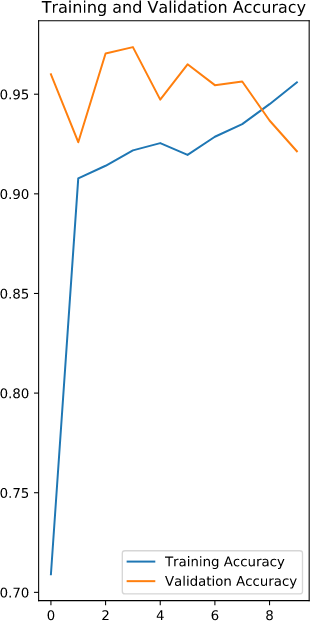
\includegraphics[width=0.5\linewidth]{images/cnn_acc_loss_1.png}
            \caption{\emph{Accuracy} par rapport au nombre d'\emph{epochs}}
    \end{subfigure}%
    \begin{subfigure}[t]{0.5\textwidth}
            \centering
            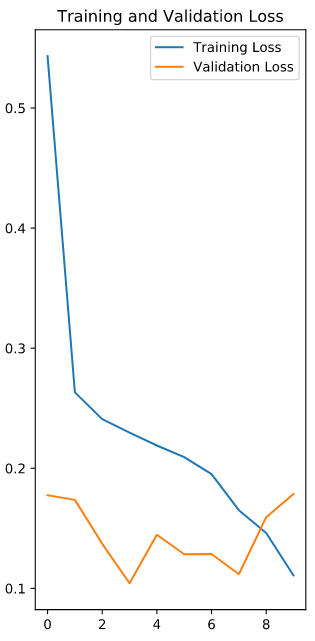
\includegraphics[width=0.5\linewidth]{images/cnn_acc_loss_2.png}
            \caption{\emph{Loss} par rapport au nombre d'\emph{epochs}}
    \end{subfigure}
    \caption{On observe une \emph{accuracy} entre 0.9 et 0.97 pour les ensembles d'images d'entraînement et de validation ainsi qu'une pente de perte descendante et proche de 0 pour les deux aussi.}
    \end{figure}

    La fonction d'erreur utilisé est $MSE = \dfrac{1}{n}\sum\limits_{y \in Y} (y - \hat{y})^2$ avec $Y$ les valeurs prédites et $\hat{y}$ leurs moyenne.
    
    \begin{figure}[H]
    \centering
    \begin{subfigure}[t]{0.5\textwidth}
            \centering
            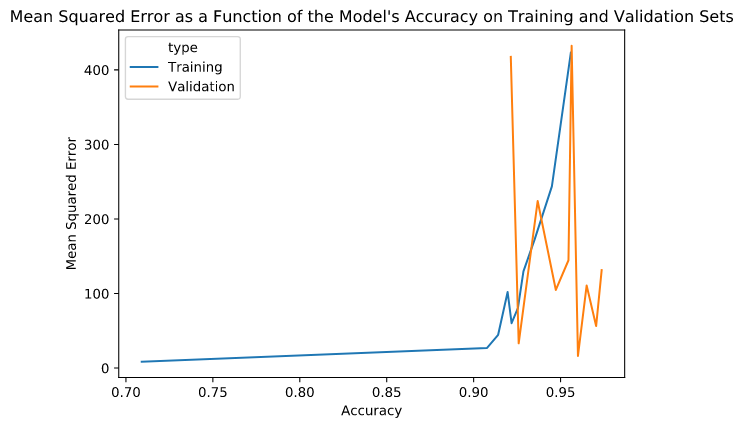
\includegraphics[width=1\linewidth]{images/cnn_mse_acc.png}
            \caption{Erreur en fonction de l'\emph{Accuracy}.}
    \end{subfigure}%
    \begin{subfigure}[t]{0.5\textwidth}
            \centering
            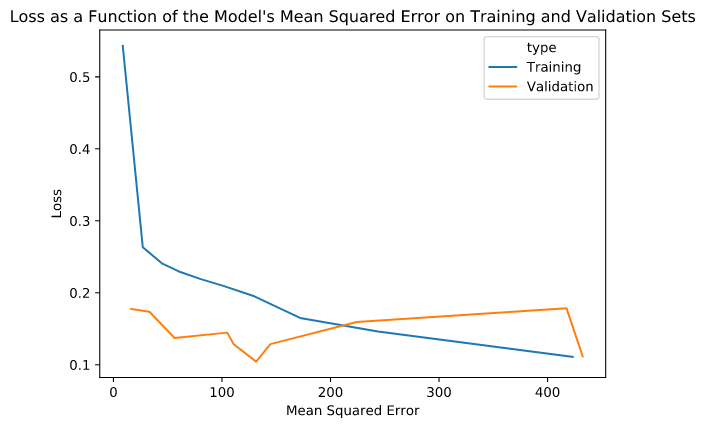
\includegraphics[width=0.95\linewidth]{images/cnn_loss_mse.png}
            \caption{Perte en fonction de l'erreur.}
    \end{subfigure}
    \caption{On constate que l'erreur varie d'une manière très irrégulière pour l'ensemble de validation et de manière exponentielle dans l'ensemble d'entraînement pour la figure A, et quand la perte converge vers 0 dans la figure B, l'erreur augmente considérablement.}
    \end{figure}
    

    L'erreur nous indique clairement que les métriques d'\emph{accuracy} et de \emph{loss} ne sont pas des indicateurs de la performance du modèle. Avec un taux d'erreur important, on peut conclure que le modèle souffre d'\emph{overfit} et qu'il n'est apte qu'à classifier les instances qu'il connaît déjà d'où les fluctuations de l'erreur pour l'ensemble de validation.
    
    \subsection{Extraction des features avec TSFresh}

      Nous avons constaté lorsque nous avons extrait les features avec TSFresh que la majorité des features les plus pertinentes étaient des coefficient de séries de Fourier.
        Nous pensons que cela est dû au fait que nos séries se généralisent très bien en des additions de sinuisoïdales. En effet, une série sans malfonctions est en réalité une répétition d'états actifs et au repos ayant une amplitude à peu près stable (en fonction du bruit); elle ressemble à un signal carré (imparfait, puisque les transitions entre les états ne sont pas instantanées).
        
        \begin{figure}[H]
            \centering
            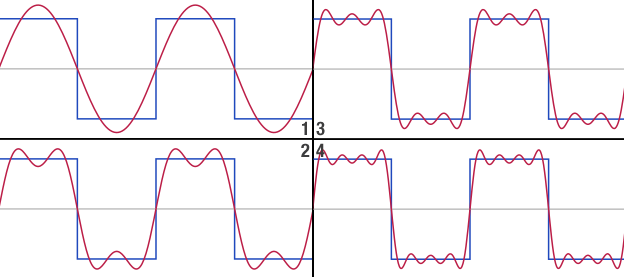
\includegraphics[width=0.75\textwidth]{images/signal_carre.png}
            \caption{Image de Wikipédia illustrant les quatre premières sommes partielles d'une série de Fourier pour approximer un signal carré.}
            \label{}
        \end{figure}
        
        En revanche, lorsque des malfonctions sont présentes dans une série, elles génèrent de plus nombreux pics haut et bas d'amplitudes à intervalles irréguliers. Ces nombreux pics empêchent d'obtenir une image relativement proche de notre courbe uniquement avec les coefficients de basse fréquence de la série de Fourier. C'est donc un indicateur simple permettant de déterminer si une série temporelle représentant la pression des senseurs présente des malfonctions ou non.
        
        Il faut cependant considérer que cela est vrai à condition que l'hypothèse que nous avons fait dans notre simulateur en fonction des données réelles auxquelles nous avons rapidement eu accès se vérifie: Les périodes des états actifs et au repos sont relativement stables. En effet, il est beaucoup plus difficile d'approximer un signal carré irrégulier avec seulement quelques coefficients d'une série de Fourier. De plus, il devient alors difficile de dissocier des pics dûs à des malfonctions de simples changement d'états anticipés.
        
    Un autre aspect est que bien que nous avons trié les features en fonction de leur pouvoir prédictif, ces tests se font de façon individuelle sur chacune des features. Or on ne peut pas exclure que certaines features soient plus ou moins efficaces dans certaines combinaisons. Ainsi, pour être sûr d'avoir l'ensemble réduit de N features le plus efficace, il faudrait tester toutes les permutations possibles et non seulement les N premiers, ce que nous n'avons pas fait pour des raisons de temps de calcul.
    
    Enfin, bien que nous ayons tenté de limiter l'\emph{overfit} autant que possible, en l'absence d'un jeu de données réel conséquent fourni par la société, nous ne pouvons être confiants de nos résultats uniquement sur les séries temporelles générées par notre simulateur.
        
        
    \subsection{Détection d'anomalies en tant qu'objets}
    Pour cette approche, on obtient des résultats intéressants. Le modèle reconnaît et isole bien les anomalies avec une bonne probabilité.
    
    \begin{figure}[H]
    \centering
    \begin{subfigure}[t]{0.3\textwidth}
            \centering
            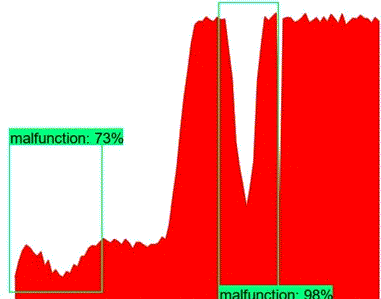
\includegraphics[width=1\textwidth]{images/od_1.png}
    \end{subfigure}%
    \begin{subfigure}[t]{0.3\textwidth}
            \centering
            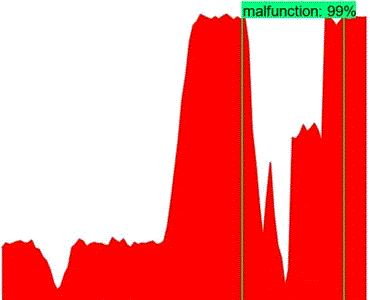
\includegraphics[width=1\textwidth]{images/od_2.png}
    \end{subfigure}
    \begin{subfigure}[t]{0.3\textwidth}
            \centering
            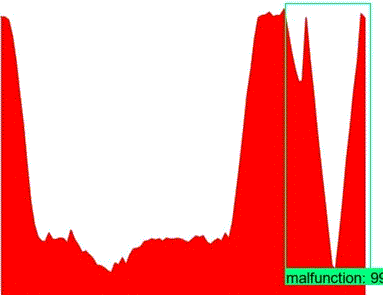
\includegraphics[width=1\textwidth]{images/od_3.png}
    \end{subfigure}
    \caption{Illustration de la détection d'anomalies sur des images différentes de celles de l'ensemble d'entraînement.}
    \end{figure}

    À l'aide de l'application de surveillance de modèles \textbf{TensorBoard}, on peut extraire quelques métriques en lien avec l'entraînement en temps réel. Cependant, l'application n'expose que des mesures de pertes et d'autres métriques qui ne sont pas documentées. Pour les mesures de perte, nous avons les résultats suivant:
    
    \begin{figure}[H]
    \centering
    \begin{subfigure}[t]{0.5\textwidth}
            \centering
            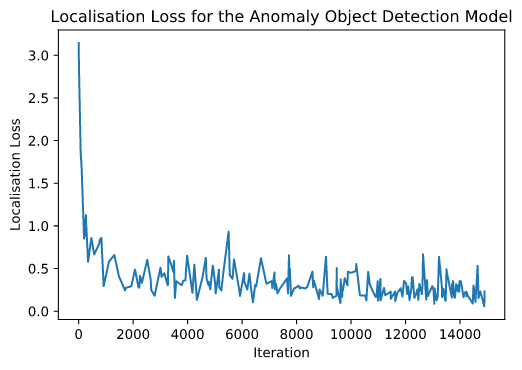
\includegraphics[width=1\textwidth]{images/od_loc_loss.png}
            \caption{Perte liée à la prédiction des coordonnées des \emph{bounding boxes} qui entourent les anomalies en fonction du nombre d'itérations écoulé.}
    \end{subfigure}%
    \begin{subfigure}[t]{0.5\textwidth}
            \centering
            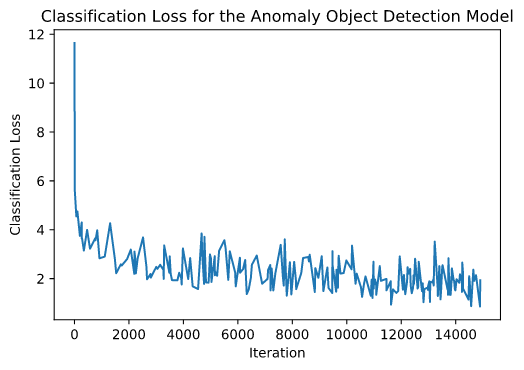
\includegraphics[width=1\textwidth]{images/od_cla_loss.png}
           	\caption{Perte liée aux prédictions de classification (la partie de l'image entourée présente-t-elle bien une anomalie ?)}
    \end{subfigure}
    \caption{Illustration de la détection d'anomalies sur des images différentes de celles de l'ensemble d'entraînement.}
    \end{figure}
    
    \begin{figure}[H]
        \centering
        \begin{subfigure}{\linewidth}
            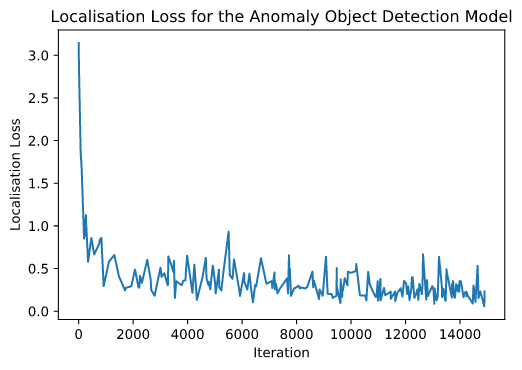
\includegraphics[width=.5\textwidth]{images/od_loc_loss.png}
            \hfill
            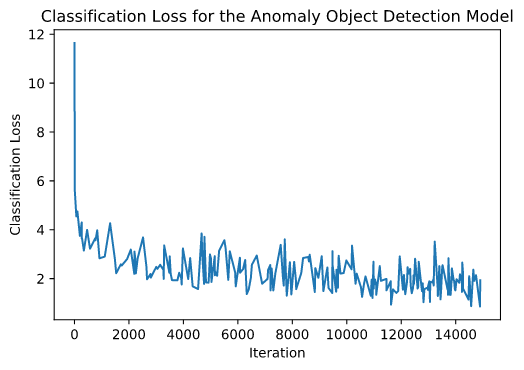
\includegraphics[width=.5\textwidth]{images/od_cla_loss.png}
        \end{subfigure}
        \caption{On observe bien une pente descendante dans les deux cas.}
    \end{figure}
    
    
    La perte de localisation est plus ou moins proche de 0, mais celle de classification est entre 1 et 2 à $15000^{\text{ème}}$ itération. Selon la documentation sur la configuration du modèle, l'\emph{API} précise qu'un nombre d'itérations de $200000$ est recommandé afin d'obtenir une perte entre 0 et 1.
    \newline
    \indent Nous n'avons pas de résultats conclusifs sur la précision et la fidélité du modèle. La perte ne nous donne pas assez d'informations comme on a pu s'en rendre compte dans le modèle CNN naïf. De plus, ni le nombre d'itérations, ni le nombre de données ne sont suffisant pour prendre en considération toutes les formes possibles d'une anomalie. Les avantages de cette approche sont tout de même à prendre en considération. L'\emph{API} de Détection d'Objets de \textit{TensorFlow} n'est pas assez documentée pour faire des expériences plus sophistiquées avec des résultats pertinents et analysables. La migration de la version 1 à la version 2 a donné naissance à plusieurs bugs ainsi que plusieurs modules obsolètes qui demandent des contournements pour fonctionner à nouveau. Il sera peut-être plus judicieux de faire jouer la concurrence et de regarder les résultats qu'on obtient avec une librairie de Deep Learning comme PyTorch qui peut est plus stable et de plus en plus adoptée.
    \newline
    \indent Néanmoins, la détection d'anomalies en temps réel est très utile au sein d'un système à temps réel. L'entreprise pourrait opter pour cette approche si sa fonctionnalité est prouvée avec des analyses et des métriques qui le montre et que nous n'avons pas eu les ressources pour réaliser.
    \section{Conclusion}

\renewcommand\refname{7\indent Références}
\begin{thebibliography}{1}
\bibitem{odwikipedia} \href{https://en.wikipedia.org/wiki/Object\_detection}{Wikipedia, Object Detection}
\bibitem{pretrainedmodel} \href{https://github.com/tensorflow/models/blob/master/research/object_detection/g3doc/detection_model_zoo.md#coco-trained-models}{TensorFlow, \textit{models} repository, Tensorflow detection model zoo.}
\bibitem{tsfreshfeatures} \href{https://tsfresh.readthedocs.io/en/latest/text/list_of_features.html}{Liste des features calculées par TSFresh, TSFresh documentation}
\end{thebibliography}
\clearpage

\section*{Glossaire}

\begin{description}  
\item [Système à temps réel] Description
\item [CNN] \textbf{C}onvolutional \textbf{N}eural \textbf{N}etwork, ou Réseau de Neurones Convolutifs est un type de réseau de neurones artificiels utilisé pour la reconnaissance d'images et autres.
\item [TensorFlow] Une librairie de Deep Learning développé par Google et écrite en Python. Elle abstrait plein de structure de données et fournit des algorithmes liés aux Deep Learning. Cette librairie permet de d'éxecuter des modèles sur le processeur ainsi que la carte graphique.
\item [Epoch] Un epoch est quand l'ensemble des données d'entraînement passe par le réseau de neurones une seule fois.
\item [Batch] Passer tout un ensemble de données 
\item [p-value] Description
\item [Object Detection] La détection d'objet est une méthode de reconnaissance d'un objet particulier dans une image.
\item [Bounding box] Région rectangulaire qui entoure un objet sur une image.
\item [CSV] \textbf{C}omma-\textbf{s}eperated \textbf{V}alues est un format spécifique regroupant des données tabulaires où chaque valeur dans un échantillon ou une ligne est séparée par une virgule.
\item [mAP] \textbf{m}ean \textbf{A}verage \textbf{P}recision est une mesure de précision utilisé dans le contexte de la détection d'objets.
\item [Fine-tuning] Le fine-tuning est une étape d'entraînement qui consiste à recalibrer les poids sur chaque connexion entre deux ou plusieurs neurones suivant l'étape du calcul de loss
\item [Loss] appelé fonction objectif en français désigne une fonction qui permet de donner une valeur à une solution pour un problème d'optimisation (optimisation des poids du réseau de neurones dans notre cas).
\item [Overfit] appelé surapprentissage en français désigne le fait qu'un modèle n'arrive pas à généraliser ses prédictions en dehors des données qu'elles lui ont été fournit lors de l'entraînement.
\end{description}


\end{document}